\clearpage
\section{Coupled analysis: MEMS cantilever beam}
In this section the MEMS cantilever beam is used to introduce
the coupled analysis features that exist. Three types of 
coupled problems are solved,
\begin{enumerate}
\item Mechanical problem
\item Thermoelastic problem
\item Electromechanical problem
\end{enumerate} 
For each, three types of analyses are conducted,
\begin{enumerate}
\item Static analysis              (\ttt{mems\_cant\_sta.m})
\item Dynamic modal analysis       (\ttt{mems\_cant\_dyn.m})
\item Transfer function evaluation (\ttt{mems\_cant\_tra.m})
\end{enumerate} 
where the file in the parantheses denotes the MATLAB execution file.
The Lua inputfiles along with the a short description of the aim of the
example is summarized in Table~\ref{table:LuaFilesForMEMSBeam}.

\begin{table}[htbp]
\centering
\caption{Lua files for a MEMS beam}
\label{table:LuaFilesForMEMSBeam}
\begin{tabular}{|l|l|l|m{2.5in}|}
\hline
Problem domain    & Lua filename                     
& MATLAB file       & Objective \\
\hhline{|=|=|=|=|}
Mechanical        & \ttt{mems\_cant\_m.lua}          
& \ttt{sta,dyn,tra} & simple mechanical problem \\
                  & \ttt{mems\_cant\_m\_nondim.lua}  
& \ttt{sta,dyn,tra} & nondimensionalization of problem \\
                  & \ttt{mems\_cant\_wa\_m.lua}      
& \ttt{sta,dyn,tra} & mechanical problem with anchor loss \\
\hline
Thermoelastic     & \ttt{mems\_cant\_te\_sta.lua}    
& \ttt{sta}         & simple static thermoelastic problem \\
                  & \ttt{mems\_cant\_te.lua}         
& \ttt{dyn,tra}     & thermoelastic problem with anchor loss \\
                  & \ttt{mems\_cant\_wa\_te\_sta.lua}
& \ttt{sta}         & static thermoelastic problem with anchor \\
                  & \ttt{mems\_cant\_wa\_te.lua}     
& \ttt{dyn,tra}     & thermoelastic problem with anchor loss \\
\hline
Electromechanical & \ttt{mems\_cant\_em.lua}         
& \ttt{sta,dyn,tra} & simple electromechanical problem \\
\hline
\end{tabular}
\end{table}

Throughout this section, the user is assumed to have worked through 
the previous two sections. Minor details of the Lua input files and 
MATLAB script files are omitted. 

\clearpage
\subsection{Mechanical analysis}
\begin{flushleft}
  \textbf{Inputfile:}
  \ttt{\ttilde/hiqlab/models/tutorial/mems\_cantilever\_beam}\\
  \textbf{Lua features introduced:}
  \ttt{mech\_nondim}(Non-dimensionalization), 
  material database in \ttt{'materials.lua'},
  \ttt{get\_dim\_scale}\\
  \textbf{MATLAB features introduced:}
  \ttt{Mesh\_get\_x, Mesh\_get\_disp, Mesh\_get\_sense\_disp,
       Mesh\_get\_u, Mesh\_get\_sense\_u, mechmode, second\_order\_bode,
       Mesh\_get\_drive\_f, Mesh\_get\_sense\_u, plot\_bode}  
\end{flushleft}
This example is used to illustrate the basic analysis methods,
the procedure for nondimensionalization and methods to extract
useful information from the analysis. A schematic of the cantilever
is shown in Figure~\ref{fig:MEMSCantileverBeam_Mech}. The beam thickness
\ttt{t} is considered to be small compared to the length \ttt{l} and
width \ttt{w}, which justifies the plane stress analysis conducted.
A point load of \ttt{P} is applied for the static analysis. For the
transfer function evaluation, the beam is forced at this tip and the
displacement is also sensed at this point.

\begin{figure}[htbp]
\centering
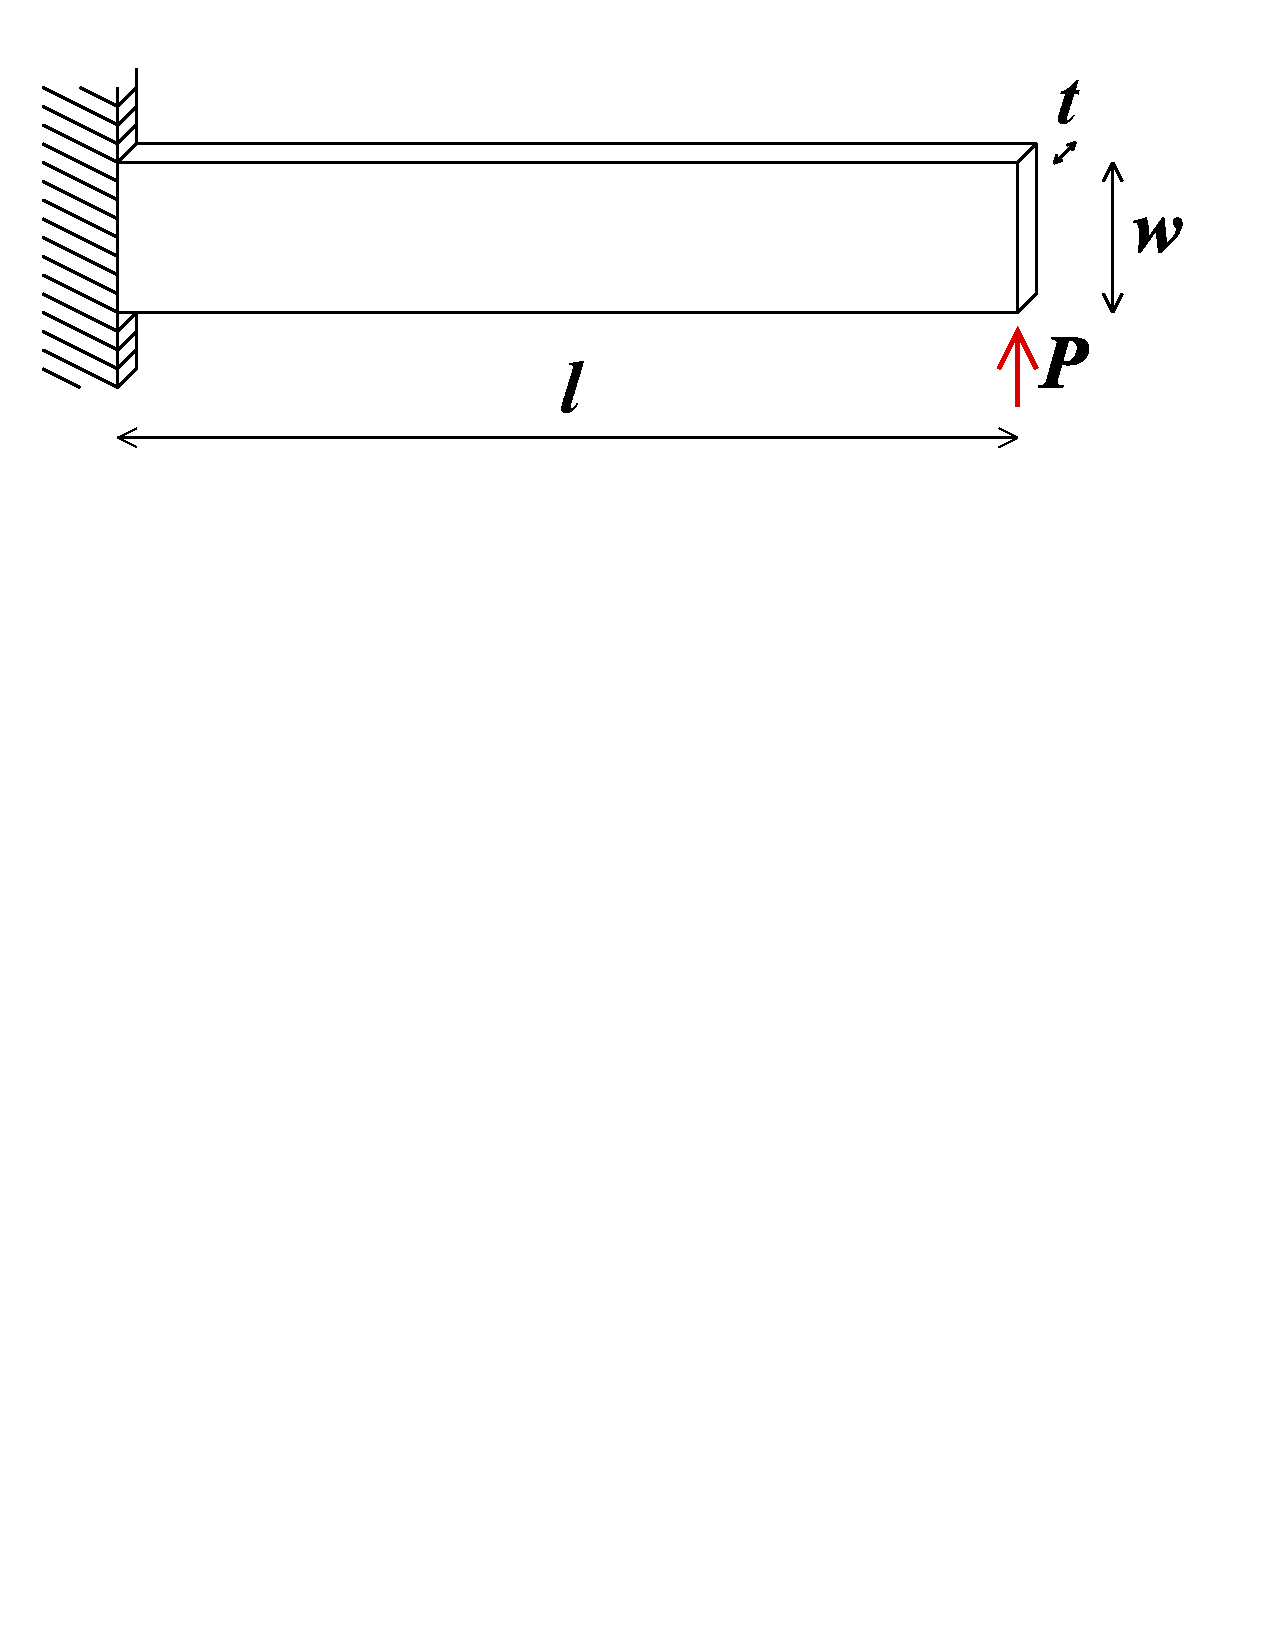
\includegraphics[trim = 0in 7in 0.5in 0in, clip, height = 2in]{fig/memscantileverbeam_mech.pdf}
\caption{Schematic of the MEMS cantilever beam}
\label{fig:MEMSCantileverBeam_Mech}
\end{figure}

\clearpage
\subsubsection*{Dimensional input file (LUA)}
\begin{flushleft}
  \textbf{Inputfile:}
  \ttt{\ttilde/hiqlab/models/tutorial/mems\_cantilever\_beam/mems\_cant\_m.lua}
\end{flushleft}
\hspace{1in}
{\footnotesize
\listinginput[10]{1}{../../../models/tutorial/mems_cantilever_beam/mems_cant_m.lua}
}

\clearpage
The analysis is conducted in dimensional form as opposed to the
Lua input file introduced in the next section.

\begin{itemize}

  \item{\textbf{Define order and approximate size of element :}}
  The default order of interpolation can be defined by a variable named
  \ttt{order}. When elements are produced by block generation without
  specification of the order of interpolation, this variable is used.
  Additionally it is convenient to set this parameter globally to
  control the interpolation of all elements.

  Similarly, the default approximate size of the elements produced by
  block generation are defined by the variable \ttt{dense}. 

  \item{\textbf{Define geometry of domain:}}
  The additional variable \ttt{t} is set for the thickness.
  Though this analysis is 2D, this variable is required to 
  define forces.

  \item{\textbf{Define force at the tip:}}
  The force is defined here not as a force per length. Thus
  when the force boundary conditions are applied, it will be
  divided by the thickness to obtain the force per unit length.  

  \item{\textbf{Define element type:}}
  Here we use the material database library. The material 
  parameters are set in the file \ttt{materials.lua} located
  in the \ttt{models} directory. See ??? for details.

\begin{verbatim}
        mtype = 'silicon2'
\end{verbatim}

  \item{\textbf{Define boundary condition:}}
  As noted above, the force boundary conditions are applied per
  unit length, since this is 2D analysis.

\begin{verbatim}
     mesheq( y, -w/2) then return ' f',  P/t; end
\end{verbatim}

  \item{\textbf{Define a sensing function to evaluate tip displacement:}}
  Displacements at nodes can be extracted by searching for the id of the
  node of interest from the nodal array. This process can be tedious when
  the number of nodes increases. As in the case of boundary conditions,
  one can extract the information of a specific node by a function of
  the form exactly the same as the boundary condition.

  The \ttt{' u'} denotes that the displacement in the $y$ direction 
  is what we would like to extract from the node. The $1$ denotes that
  we would like this value multiplied by unity. By invoking this function
  through MATLAB, a sensing vector is produced, with which the inner 
  product with displacement vector results in the desired quantity. 

  \item{\textbf{Define a sensing and forcing functions for producing 
                                                      a bode plott:}}
  As in the prevous function definition, these functions are used to 
  define the forcing and sensing patterns used to generate the bode plot.

  In the definition of the force function, the force $P$ has again been
  modified appropriately to reflect the 2D analysis.

\end{itemize}


\clearpage
\subsubsection*{Construct non-dimensional input file (LUA)}
\begin{flushleft}
  \textbf{Inputfile:}
  \ttt{\ttilde/hiqlab/models/tutorial/mems\_cantilever\_beam/mems\_cant\_m\_nondim.lua}\\
\end{flushleft}
\hspace{1in}
{\footnotesize
\listinginput[10]{1}{../../../models/tutorial/mems_cantilever_beam/mems_cant_m_nondim.lua}
}

\clearpage
The input file for the MEMS cantilever for analysis in nondimensional 
form is presented. The user can observe that the difference between the 
dimensional case is subtle. Below the differences are explained.

\begin{itemize}

  \item{\textbf{Define nondimensionalization parameters:}}
  Nondimensionalization is defined through the function \ttt{mech\_nondim}. 
  \begin{verbatim}
      -- Define nondimensionalization parameters
      mech_nondim('silicon2',7e-6)
  \end{verbatim}
  The first argument defines the material parameters used to define 
  the characteristic parameters; The second defines the characteristic 
  length scale. Dimensional parameters can also be set manually by
  directly manipulating the table \ttt{dim\_scales} which contain these
  constants.(See section on non-dimensionalization for details).

  \item{\textbf{Define boundary condition:}}
  As noted above, in 2D analysis the force boundary conditions are applied per
  unit length. The nondimensionalization does not
  take into account the 2D analysis feature, that the forces should be 
  per unit length. Thus forces when given, must be given in terms of 
  force per normalized unit length.
  \begin{verbatim}
      mesheq( y, -w/2) then return ' f',  P/t*get_dim_scale('L'); end
  \end{verbatim}

  The function \ttt{get\_dim\_scale} returns the characteristic scale 
  for \ttt{'L'} which is the length scale. The number returned is 
  extracted from a table defined as \ttt{dim\_scales}. See section on
  non-dimensionalization for details.

\end{itemize}
\clearpage
\subsubsection*{Construct non-dimensional input file (Beam with anchors)(LUA)}
\begin{flushleft}
  \textbf{Inputfile:}
  \ttt{\ttilde/hiqlab/models/tutorial/mems\_cantilever\_beam/mems\_cant\_wa\_m.lua}\\
\end{flushleft}
\hspace{1in}
{\footnotesize
\listinginput[10]{1}{../../../models/tutorial/mems_cantilever_beam/mems_cant_wa_m.lua}
}

\clearpage
The input file for the MEMS cantilever beam with anchors is 
presented. The only difference with the previous input file
is the use of the function \ttt{pml\_blocks2d}, which constructs
an anchor and returns the appropriate boundary conditions and
stretch function.
\begin{itemize}

  \item{\textbf{Construct anchor:}}
  The \ttt{pml\_blocks2d} function frees the user from the tedium
  of meshing the anchor block and generating appropriate boundary
  condition functions and stretch functions.
  \begin{verbatim}
      bc_func, st_func = pml_blocks2d({0,0},{w/2,-w/2},2,Pw,Ph,Pd,
                                      f0,etype,order,dense,dense)
  \end{verbatim}


\end{itemize}

\clearpage
\subsubsection*{Solve static problem (MATLAB)}
\begin{flushleft}
  \textbf{Inputfile:}
  \ttt{\ttilde/hiqlab/models/tutorial/mems\_cantilever\_beam/mems\_cant\_sta.m}\\
\end{flushleft}
\hspace{1in}
{\footnotesize
\listinginput[10]{1}{../../../models/tutorial/mems_cantilever_beam/mems_cant_sta.m}
}

\clearpage
This script extracts the displacement at the tip in 3 different methods. 
The method using sensing functions is strongly recommended.

\begin{itemize}

  \item{\textbf{Obtain tip displacements(MATLAB)}}
  This method shows the crude way of extracting the displacement
  at the tip. First the nodal array is obtained. Then variables
  \ttt{l} and \ttt{w} defining the length and width of the beam 
  are extracted from the Lua environment. From this, the tip nodes 
  are obtained by the \ttt{find} command in MATLAB.

  Next the displacement vector at the nodes are extracted. Finally 
  the displacement in the second direction at the node is found.

  \item{\textbf{Obtain tip displacements through 
                                    \ttt{Mesh\_get\_sense\_disp}}}
  This method is slightly more efficient. The sense vector is obtained 
  at each node by the function \ttt{Mesh\_get\_sense\_disp}. This 
  returns sense vector which is unreduced, i.e., has entries from each 
  degree of freedom at each node. This vector is contracted with the 
  displacement vector to obtain the displacement at the node.

  \item{\textbf{Obtain tip displacements through \ttt{Mesh\_get\_sense\_u}}}
  This is the method that is most recommended if the node of interest 
  is a free degree of freedom.  The function \ttt{Mesh\_get\_sense\_u} 
  returns a sense vector in reduced form, containing only the free 
  degrees of freedom. This is contracted with the $U$ vector which also 
  contains only the free degrees of freedom to obtain the desired 
  displacement.

\end{itemize}

In the case where the nondimensionalized input file is used, nothing 
needs to be modified for the MATLAB script file which is used to solve 
the problem. The only thing that one must be aware of is which functions 
return dimensional quantaties from the mesh. This is noted in the 
section concerning non-dimensionalization.

The results obtained for the three input files are shown in 
Figures 
\ref{fig:MEMSCantileverBeamMesh},
\ref{fig:MEMSCantileverBeamWaMesh},
\ref{fig:MEMSCantileverBeamStatic},
\ref{fig:MEMSCantileverBeamWaStatic}.
The top two figures show the mesh for the no-anchor and anchor
case, and the bottom two figures show their static deflections.
Only one result is presented for the non-anchor case since
the dimensional and non-dimensional case return the same 
results. 

Though convergence of the solution is not obtained at this
mesh, the tip displacements are presented for reference.
\begin{verbatim}
Tip displacement for no-anchor :6.860000e-09
Tip displacement for    anchor :8.227792e-09
\end{verbatim}


\begin{figure}[htbp]
\begin{minipage}{0.45\linewidth}
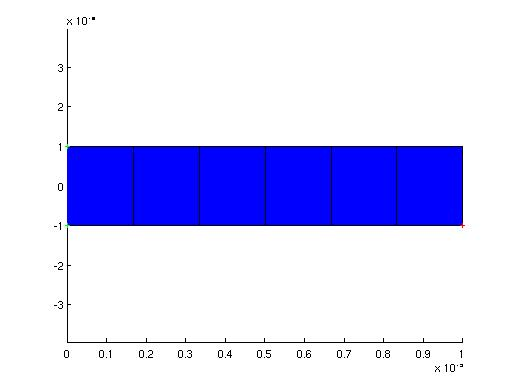
\includegraphics[height = 2in]{fig/mems_cant_m_mesh.jpg}
\caption{Mesh for a MEMS cantilever beam}
\label{fig:MEMSCantileverBeamMesh}
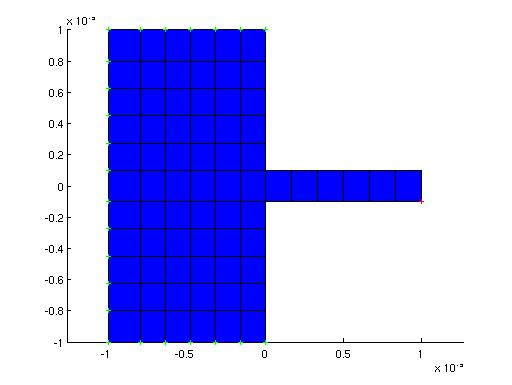
\includegraphics[height = 2in]{fig/mems_cant_wa_m_mesh.jpg}
\caption{Mesh for a MEMS cantilever beam with anchor}
\label{fig:MEMSCantileverBeamWaMesh}
\end{minipage}
\hfill
\begin{minipage}{0.45\linewidth}
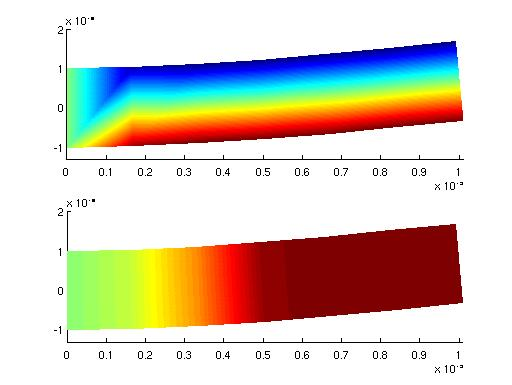
\includegraphics[height = 2in]{fig/mems_cant_m_sta.jpg}
\caption{Static deformation of a MEMS cantilever beam}
\label{fig:MEMSCantileverBeamStatic}
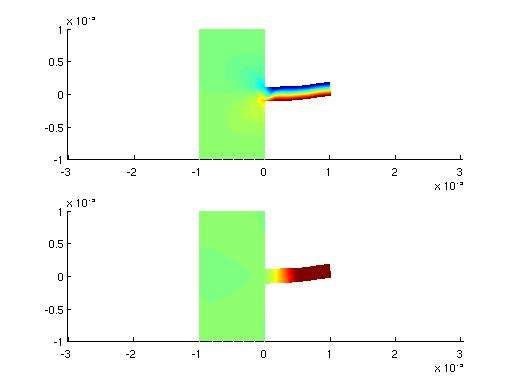
\includegraphics[height = 2in]{fig/mems_cant_wa_m_sta.jpg}
\caption{Static deformation of a MEMS cantilever beam with anchor}
\label{fig:MEMSCantileverBeamWaStatic}
\end{minipage}
\end{figure}



\clearpage
\subsubsection*{Solve dynamic modal problem (MATLAB)}
\begin{flushleft}
  \textbf{Inputfile:}
  \ttt{\ttilde/hiqlab/models/tutorial/mems\_cantilever\_beam/mems\_cant\_dyn.m}\\
\end{flushleft}
\hspace{1in}
{\footnotesize
\listinginput[10]{1}{../../../models/tutorial/mems_cantilever_beam/mems_cant_dyn.m}
}

\clearpage
The script conducts modal analysis and extracts the modes and 
frequencies of the beam.

\begin{itemize}

  \item{\textbf{Solve dynamic problem}}
  The variable \ttt{w0} defines the approximate value of the frequency 
  in radians that we are interested in. In this case we specify zero to 
  find those that are the smallest. \ttt{nev} eigenfrequencies are sought. 
  These are obtained by the function \ttt{mechmode}. The function returns 
  the mode shape, frequency[rad/s] and the $Q$. In this case, we have 
  not incorporated any damping and results will give us close to 
  infinite $Q$ values. For the case of anchor loss, a nonzero \ttt{w0}
  is given, since zero would not give the first bending mode as a result.

\end{itemize}

In the case where the nondimensionalized input file is used, nothing 
needs to be modified for the MATLAB script file which is used to solve 
the problem. The only thing that one must be aware of is which functions 
return dimensional quantaties from the mesh. This is noted in the section 
concerning non-dimensionalization.

The results obtained for the three input files are shown in 
Figures 
\ref{fig:MEMSCantileverBeamDynamic},
\ref{fig:MEMSCantileverBeamWaDynamic}.
The two figures show the mode obtained for the first bending mode
of the structure. 
Again, only one result is presented for the non-anchor case since
the dimensional and non-dimensional case return the same 
results. 

Though convergence of the solution is not obtained at this
mesh, the results are presented for reference.
\begin{verbatim}
No-anchor
------------------------------
Freq [Hz]   :3.101849e+07
            :2.181131e-07
Q           :7.110644e+13

Anchor
------------------------------
Freq [Hz]   :2.737977e+07
            :7.727477e+04
Q           :1.771592e+02
\end{verbatim}

\begin{figure}
\centering
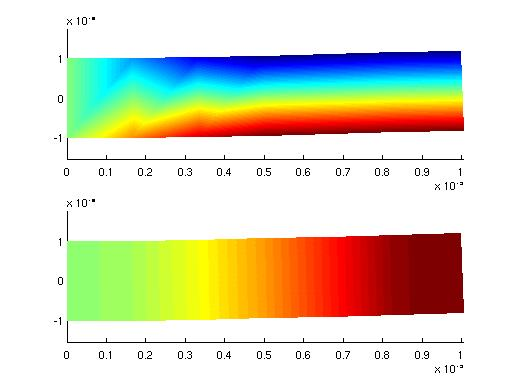
\includegraphics[height = 2in]{fig/mems_cant_m_dyn.jpg}
\caption{Dynamic mode of a MEMS cantilever beam}
\label{fig:MEMSCantileverBeamDynamic}
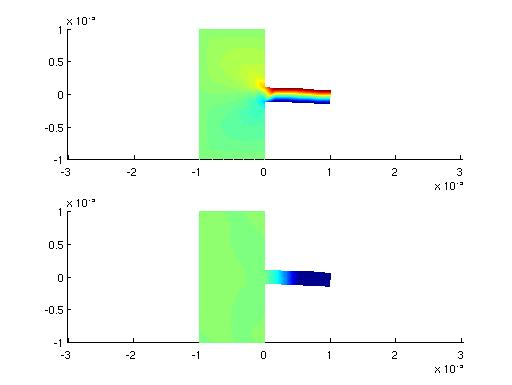
\includegraphics[height = 2in]{fig/mems_cant_wa_m_dyn.jpg}
\caption{Dynamic mode of a MEMS cantilever beam with anchor}
\label{fig:MEMSCantileverBeamWaDynamic}
\end{figure}


\clearpage
\subsubsection*{Solve for transfer function (MATLAB)}
\begin{flushleft}
  \textbf{Inputfile:}
  \ttt{\ttilde/hiqlab/models/tutorial/mems\_cantilever\_beam/mems\_cant\_tra.m}\\
\end{flushleft}
\hspace{1in}
{\footnotesize
\listinginput[10]{1}{../../../models/tutorial/mems_cantilever_beam/mems_cant_tra.m}
}

\clearpage
The script computes the transfer function between the force and 
displacement at the tip.

\begin{itemize}

  \item{\textbf{Compute forcing and sensing vectors}}
  The forcing and sensing vectors required for the transfer function 
  evaluation are obtained by the \ttt{Mesh\_get\_sense\_u} and 
  \ttt{Mesh\_get\_drive\_f} functions.

  \item{\textbf{Solve for transfer function}}
  \ttt{second\_order\_bode} is used to compute the transfer function.
  The range of the frequency that we would like to sweep across are 
  specified here. The variable \ttt{wc} defines the center frequency 
  of the sweep in [rad/s]. that we are interested in. The response and 
  frequency in [rad/s] are returned.

  \item{\textbf{Show bode plot}}
  The function \ttt{plot\_bode} is used to visualize the results.

\end{itemize}

In the case where the nondimensionalized input file is used, nothing 
needs to be modified for the MATLAB script file which is used to solve 
the problem. The only thing that one must be aware of is which functions 
return dimensional quantaties from the mesh. This is noted in the 
section concerning non-dimensionalization.

The results obtained for the three input files are shown in 
Figures 
\ref{fig:MEMSCantileverBeamTransfer},
\ref{fig:MEMSCantileverBeamWaTransfer}.
The two figures show the transfer function obtained for
the no-anchor and anchor case.
Again, only one result is presented for the non-anchor case since
the dimensional and non-dimensional case return the same 
results. 

Though convergence of the solution is not obtained at this
mesh, the results are presented for reference.

\begin{figure}
\centering
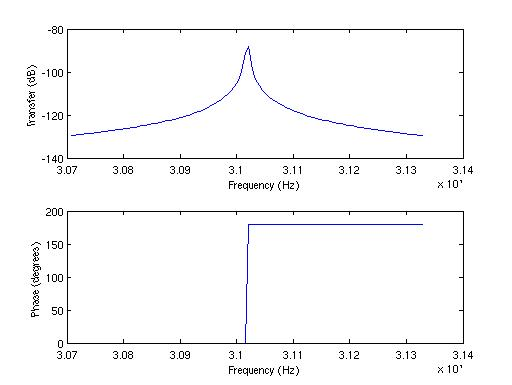
\includegraphics[height = 2in]{fig/mems_cant_m_tra.jpg}
\caption{Transfer function of a MEMS cantilever beam}
\label{fig:MEMSCantileverBeamTransfer}
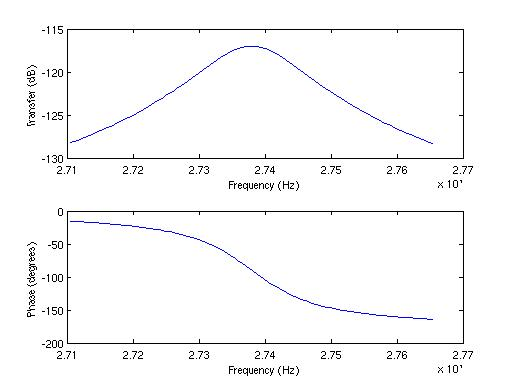
\includegraphics[height = 2in]{fig/mems_cant_wa_m_tra.jpg}
\caption{Transfer function of a MEMS cantilever beam with anchor}
\label{fig:MEMSCantileverBeamWaTransfer}
\end{figure}


\clearpage
\subsection{Thermomechanical analysis}
\begin{flushleft}
  \textbf{Inputfile:}
  \ttt{\ttilde/hiqlab/models/tutorial/mems\_cantilever\_beam}\\
  \textbf{Lua features introduced:}
  \ttt{ted\_nondim}\\
  \textbf{MATLAB features introduced:}
  \ttt{tedmode}
\end{flushleft}
This example is used to illustrate the analysis of the
thermo-mechanical response of a MEMS cantilever beam. For the coupled 
problem, the characteristic scales that govern the individual 
fields can vary greatly. Due to this fact, non-dimensionalization
should always be incorporated. For the thermoelastic case, this
can easily be done by defining the \ttt{ted\_nondim} function.

In this section, a differential temperature is applied to the
top and bottom of the beam to compute the static deflection
under this load. A schematic of this is shown in 
Figure~\ref{fig:MEMSCantileverBeam_Te_Sta}.
The modal analysis and transfer function response of this cantilever
beam in the configuration shown in 
Figure~\ref{fig:MEMSCantileverBeam_Mech} is also analyzed.

\begin{figure}[htbp]
\centering
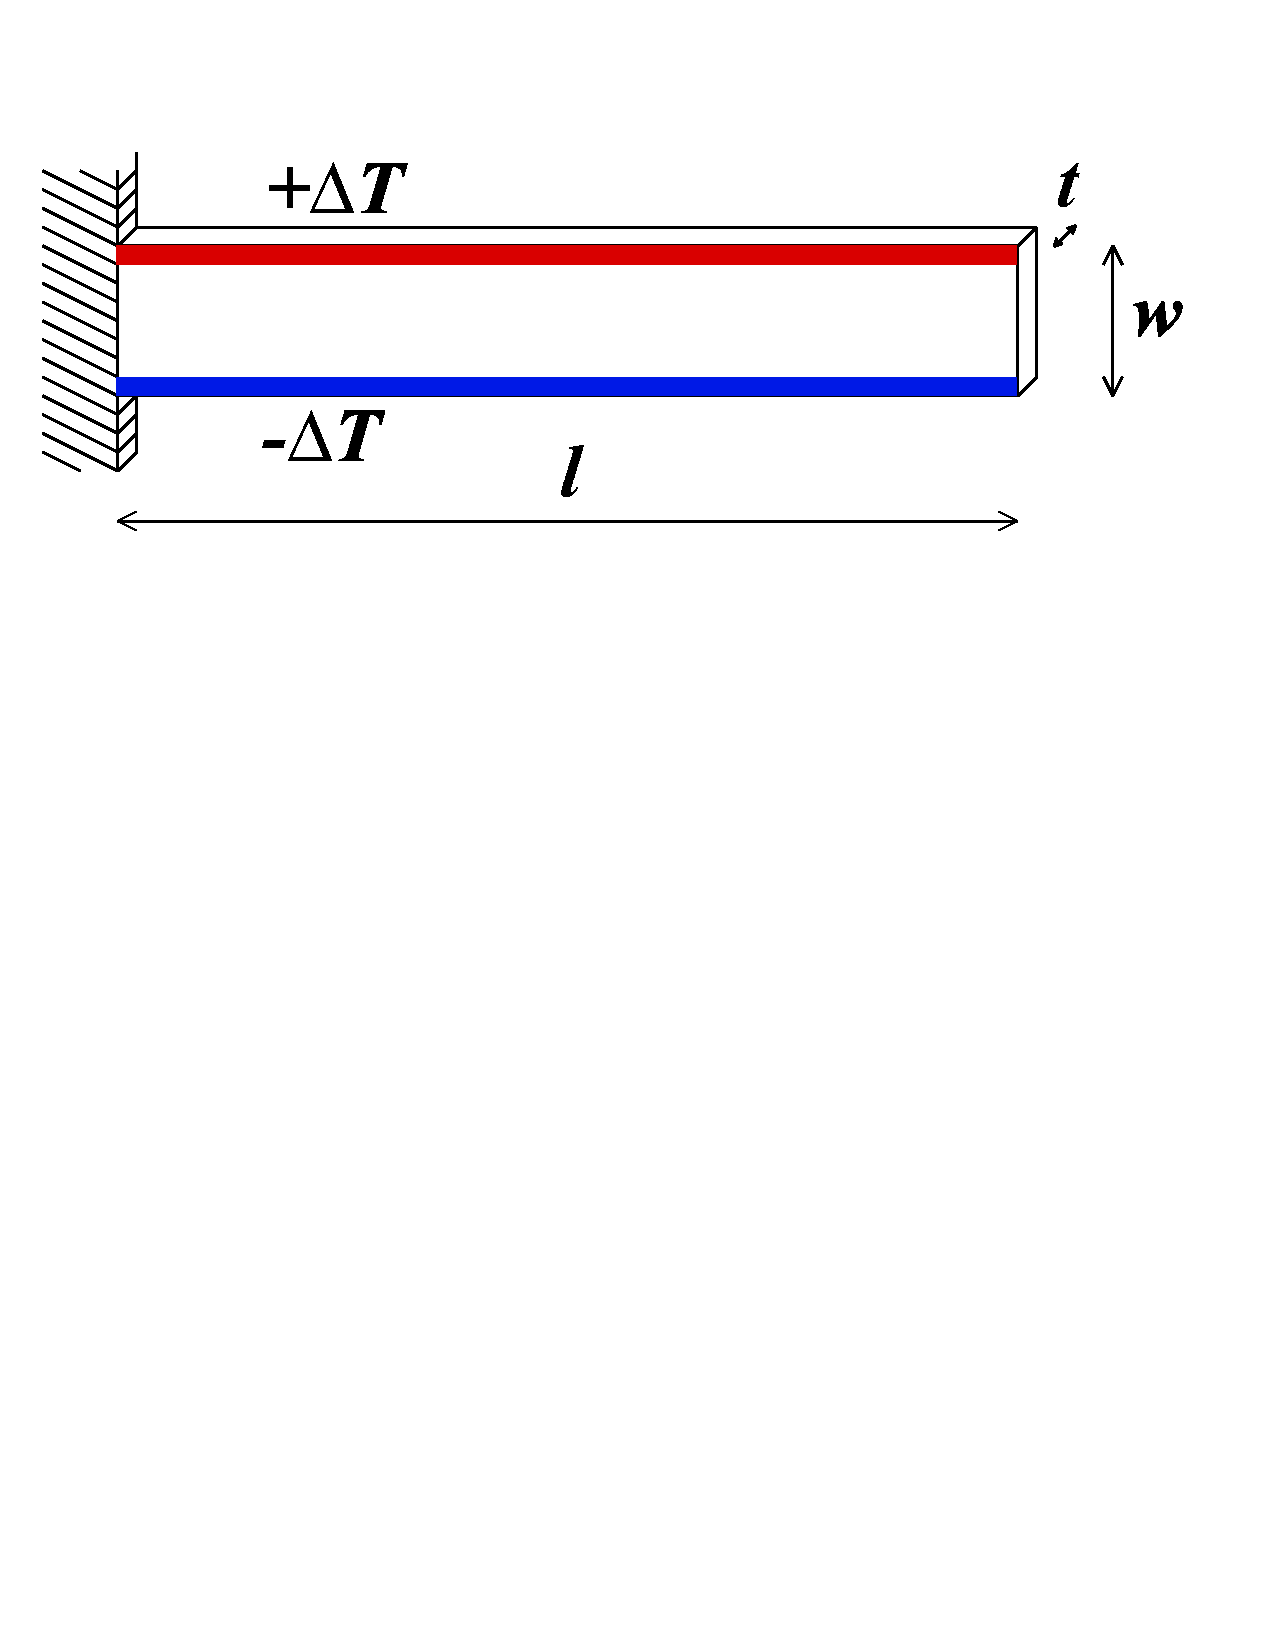
\includegraphics[trim = 0in 7in 0.5in 0in, clip, height = 2in]{fig/memscantileverbeam_te_sta.pdf}
\caption{Schematic of the MEMS cantilever beam (Thermoelastic static case)}
\label{fig:MEMSCantileverBeam_Te_Sta}
\end{figure}

\clearpage
\subsubsection*{Input file for static case (LUA)}
\begin{flushleft}
  \textbf{Inputfile:}
  \ttt{\ttilde/hiqlab/models/tutorial/mems\_cantilever\_beam/mems\_cant\_te\_sta.lua}\\
\end{flushleft}
\hspace{1in}
{\footnotesize
\listinginput[10]{1}{../../../models/tutorial/mems_cantilever_beam/mems_cant_te_sta.lua}
}

\clearpage
\begin{itemize}

  \item{\textbf{Define nondimensionalization parameters:}}
  Nondimensionalization is defined through the function \ttt{ted\_nondim}. 
  \begin{verbatim}
      -- Define nondimensionalization parameters
      ted_nondim('silicon2',7e-6)
  \end{verbatim}
  The first argument defines the material parameters used to define 
  the characteristic parameters; The second defines the characteristic 
  length scale.
  
  \item{\textbf{Define element type:}}
  For this analysis, a thermoelastic element is required. This can be 
  constructed by the function,
  \begin{verbatim}
      etype = make_material_te(mtype, 'planestress')
  \end{verbatim}

  \item{\textbf{Define boundary condition:}}
  For this case a constant temperature of 10 is applied to the top part 
  of the beam, and -10 to the bottom. The beam is fixed mechanically at 
  the left end.

\end{itemize}

\clearpage
\subsubsection*{Input file for dynamic modal and transfer function (LUA)}
\begin{flushleft}
  \textbf{Inputfile:}
  \ttt{\ttilde/hiqlab/models/tutorial/mems\_cantilever\_beam/mems\_cant\_te.lua}\\
\end{flushleft}
\hspace{1in}
{\footnotesize
\listinginput[10]{1}{../../../models/tutorial/mems_cantilever_beam/mems_cant_te.lua}
}

\clearpage
\subsubsection*{Solve static problem (MATLAB)}
Once the mesh is defined, the next step is to solve the problem.
Since this script is identical to the mechanical case we will only 
explain the parameters that are set.
\begin{itemize}

  \item{\textbf{Setting parameters:}}

\end{itemize}

\begin{figure}[htbp]
\begin{minipage}{0.45\linewidth}
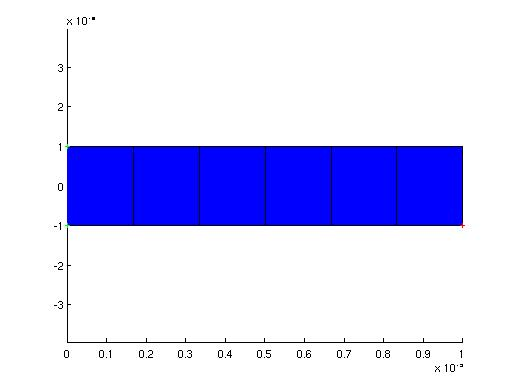
\includegraphics[height = 2in]{fig/mems_cant_m_mesh.jpg}
\caption{Mesh for a MEMS cantilever beam}
\label{fig:MEMSCantileverBeamTEMesh}
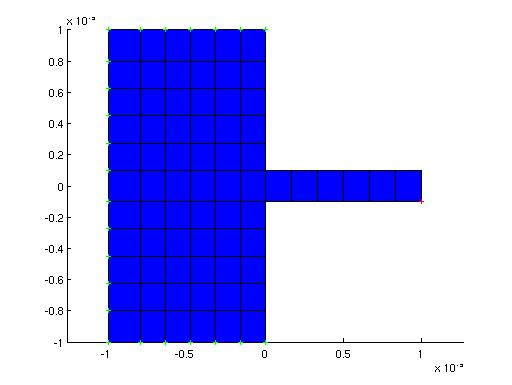
\includegraphics[height = 2in]{fig/mems_cant_wa_m_mesh.jpg}
\caption{Mesh for a MEMS cantilever beam with anchor}
\label{fig:MEMSCantileverBeamWaTEMesh}
\end{minipage}
\hfill
\begin{minipage}{0.45\linewidth}
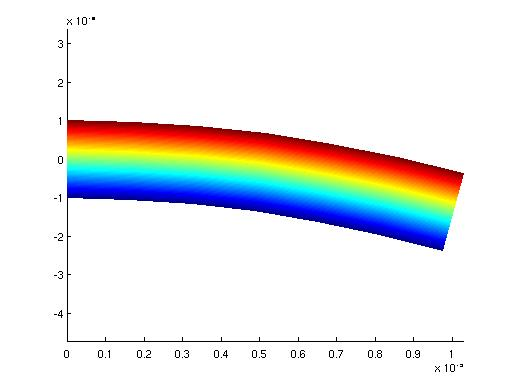
\includegraphics[height = 2in]{fig/mems_cant_te_sta.jpg}
\caption{Static deformation of a MEMS cantilever beam}
\label{fig:MEMSCantileverBeamTEStatic}
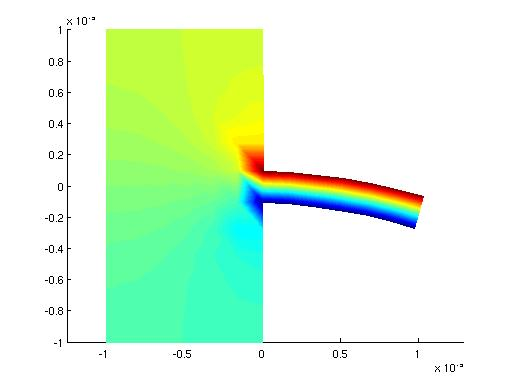
\includegraphics[height = 2in]{fig/mems_cant_wa_te_sta.jpg}
\caption{Static deformation of a MEMS cantilever beam with anchor}
\label{fig:MEMSCantileverBeamWaTEStatic}
\end{minipage}
\end{figure}

Results obtained were,
\begin{verbatim}
Tip displacement y:-1.359553e-09

Tip displacement y:-1.699258e-09
\end{verbatim}

\clearpage
\subsubsection*{Solve dynamic problem (MATLAB)}
Once the mesh is defined, the next step is to solve the problem.
Since this script is identical to the mechanical case we will only 
explain the parameters that are set.
\begin{itemize}

  \item{\textbf{Setting parameters:}}

\end{itemize}
Compared to the mechanical problem the value for \ttt{w0} is set to a
nonzero value. If \ttt{w0} were set to zero, there is a large possibility
that we would not obtain the mode of interest. By giving a close estimate
of the frequency of the mode of interest, the desired mode will be 
obtained with higher probability. This estimate \ttt{w0} may be obtained
from the purely mechanical analysis.

\begin{figure}
\centering
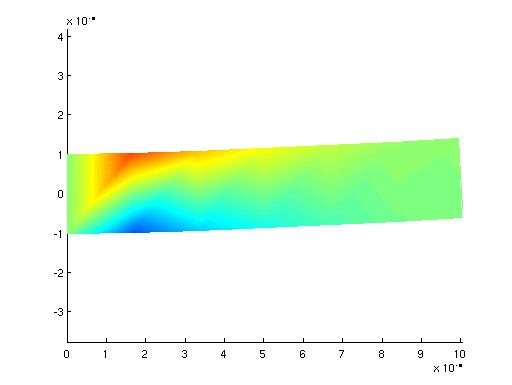
\includegraphics[height = 2in]{fig/mems_cant_te_dyn.jpg}
\caption{Dynamic mode of a MEMS cantilever beam}
\label{fig:MEMSCantileverBeamTEDynamic}
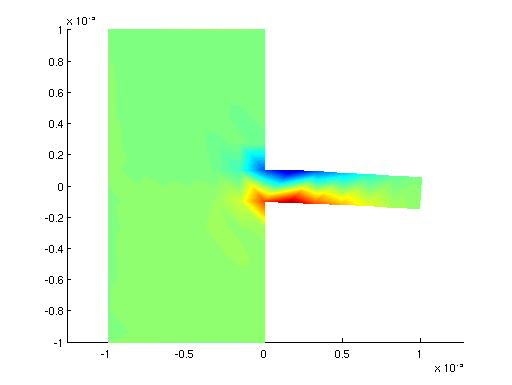
\includegraphics[height = 2in]{fig/mems_cant_wa_te_dyn.jpg}
\caption{Dynamic mode of a MEMS cantilever beam with anchor}
\label{fig:MEMSCantileverBeamWaTEDynamic}
\end{figure}

Results obtained were,
\begin{verbatim}
Freq [Hz]   :3.102175e+07
            :1.043208e+03
Q           :1.486844e+04

Freq [Hz]   :2.738287e+07
            :7.820706e+04
Q           :1.750672e+02
\end{verbatim}

\clearpage
\subsubsection*{Solve for transfer function  (MATLAB)}
Once the mesh is defined, the next step is to solve the problem.
Since this script is identical to the mechanical case we will only 
explain the parameters that are set.
\begin{itemize}

  \item{\textbf{Setting parameters:}}

\end{itemize}

\begin{figure}
\centering
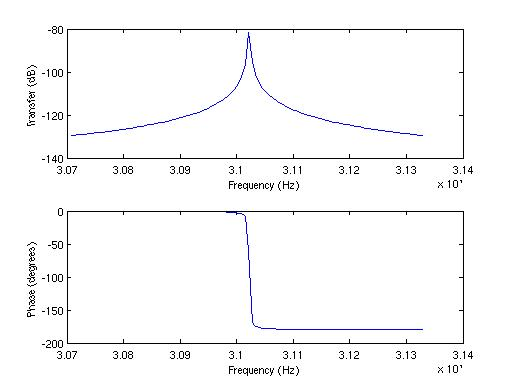
\includegraphics[height = 2in]{fig/mems_cant_te_tra.jpg}
\caption{Transfer function of a MEMS cantilever beam}
\label{fig:MEMSCantileverBeamTETransfer}
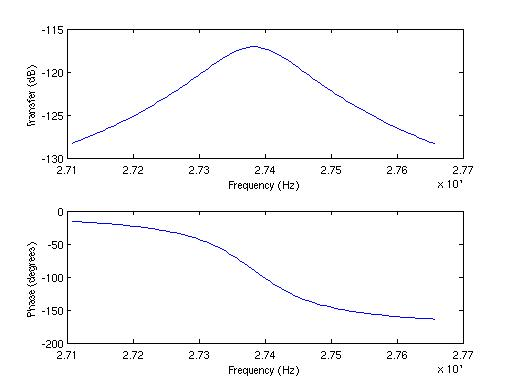
\includegraphics[height = 2in]{fig/mems_cant_wa_te_tra.jpg}
\caption{Transfer function of a MEMS cantilever beam with anchor}
\label{fig:MEMSCantileverBeamWaTETransfer}
\end{figure}




\clearpage
\subsection{Electromechanical analysis}
\begin{flushleft}
  \textbf{Inputfile:}
  \ttt{\ttilde/hiqlab/models/tutorial/mems\_cantilever\_beam}\\
  \textbf{Lua functions used:}
\end{flushleft}
This example is used to illustrate the analysis of the
electro-mechanical response of a mems beam. For the coupled
problem, the characteristic scales that govern the individual
fields can vary greatly. Due to this fact, non-dimensionalization
should always be incorporated. For the electromechanical case, this
can easily be done by defining the \ttt{em\_nondim} function.

In this section, a voltage difference will be applied between the 
beam and the substrate. to compute the static deflection
under this load. Also, the dynamic response of this cantilever
beam, both the eigenvalues and transfer function response will
be evaluated. The model reduction technique for the electromechanical
problem will also be introduced.

\begin{figure}[htbp]
\centering
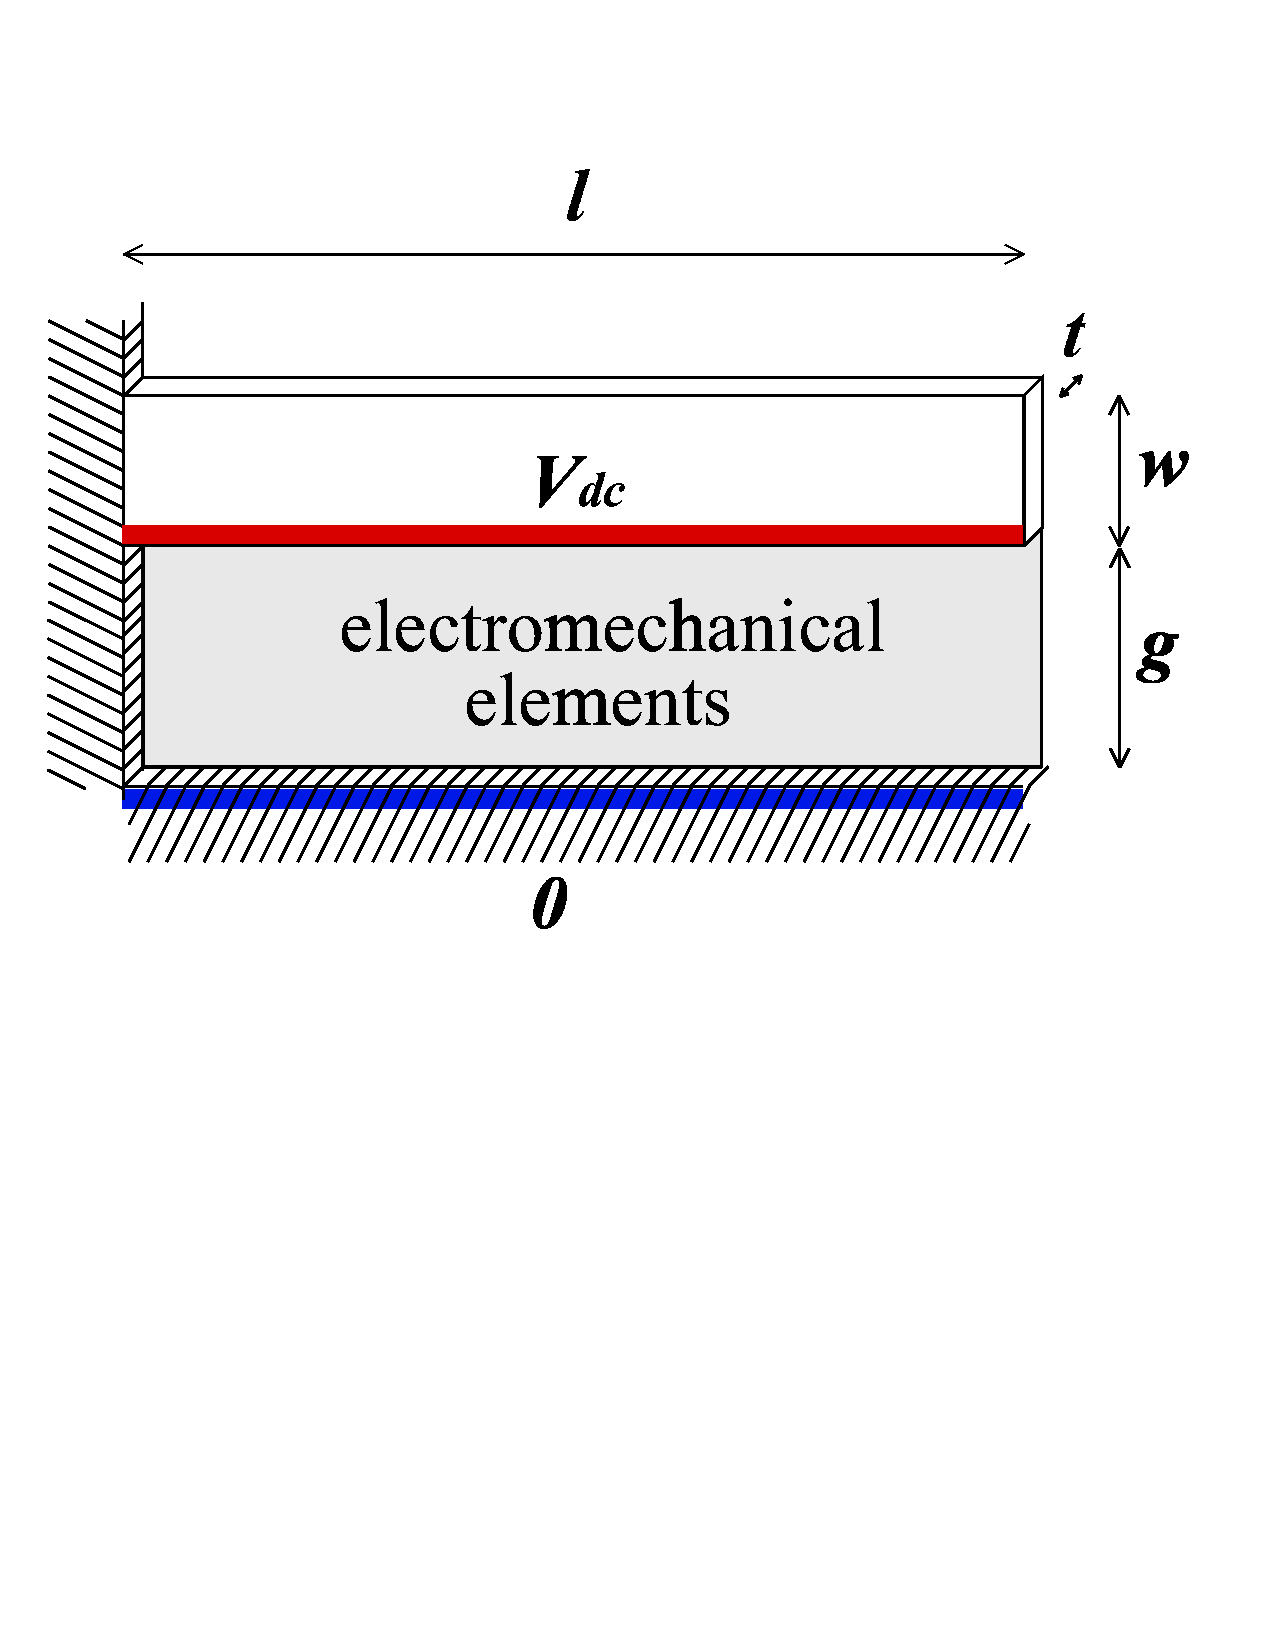
\includegraphics[trim = 0in 4in 0.5in 0in, clip, height = 2in]{fig/memscantileverbeam_em.pdf}
\caption{Schematic of the MEMS cantilever beam 
                              (Electromechanical static case)}
\label{fig:MEMSCantileverBeam_EM}
\end{figure}

\clearpage
\subsubsection*{Input file (LUA)}
\begin{flushleft}
  \textbf{Inputfile:}
  \ttt{\ttilde/hiqlab/models/tutorial/mems\_cantilever\_beam/mems\_cant\_em.lua}\\
\end{flushleft}
\hspace{1in}
{\footnotesize
\listinginput[10]{1}{../../../models/tutorial/mems_cantilever_beam/mems_cant_em.lua}
}

\clearpage
\begin{itemize}

  \item{\textbf{Define nondimensionalization parameters:}}
  Nondimensionalization is defined through the function \ttt{em\_nondim}.
  \begin{verbatim}
      -- Define nondimensionalization parameters
      em_nondim('silicon2',7e-6)
  \end{verbatim}
  The first argument defines the material parameters used to define 
  the characteristic parameters; The second defines the characteristic 
  length scale.

  \item{\textbf{Define element type:}}
  For this analysis, an electromechanical element is required besides 
  the elastic element. This can be constructed by the function,
  \begin{verbatim}
      etype = make_material_em(get_dim_scale('eps')*reps, 'planestress')
  \end{verbatim}
  By using the \ttt{get\_dim\_scale} function, the value of the 
  permitiviyt of free space can be extracted from the table 
  \ttt{dim\_scales}. 

  \item{\textbf{Define mesh using block command:}}
  Besides the mechanical beam, place electromechanical elements between 
  the underlying substrate and beam. Care must be taken in placing element 
  so that only one element is
  placed in this gap. Placing more than one element will introduce 
  hanging nodes.

  \item{\textbf{Define boundary condition:}}
  The beam is fixed mechanically at the left end. All mechanical 
  displacements within the gap are fixed to zero. A voltage of \ttt{V} 
  is applied to the beam and zero to the substrate through the 
  funtion \ttt{gap\_v\_bc}.

\end{itemize}

\clearpage
\subsubsection*{Solve static problem (MATLAB)}
Once the mesh is defined, the next step is to solve the problem.
Since this script is identical to the mechanical case we will only
explain the parameters that are set.
\begin{itemize}

  \item{\textbf{Setting parameters:}}

\end{itemize}
Since this electromechanical problem is nonlinear in the gap, 
a nonlinear iterative solve must be conducted. This is specified by 
the argument passed to the function \ttt{static\_state.m}.

Results obtained were,
\begin{verbatim}
Tip displacement y:-1.142867e-10
\end{verbatim}

\begin{figure}[htbp]
\centering
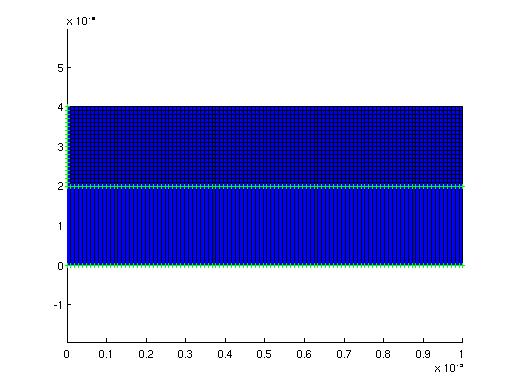
\includegraphics[height = 2in]{fig/mems_cant_em_mesh.jpg}
\caption{Mesh for a MEMS cantilever beam}
\label{fig:MEMSCantileverBeamEMMesh}
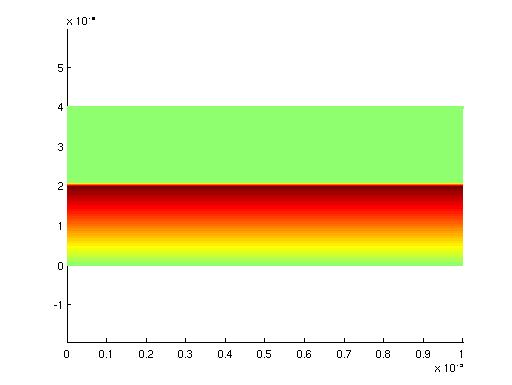
\includegraphics[height = 2in]{fig/mems_cant_em_sta.jpg}
\caption{Static deformation of a MEMS cantilever beam}
\label{fig:MEMSCantileverBeamEMStatic}
\end{figure}



\clearpage
\subsubsection*{Solve dynamic problem (MATLAB)}
Once the mesh is defined, the next step is to solve the problem.
Since this script is identical to the mechanical case we will only
explain the parameters that are set.
\begin{itemize}

  \item{\textbf{Setting parameters:}}

\end{itemize}
Compared to the mechanical problem the value for \ttt{w0} is set to a
nonzero value. If \ttt{w0} were set to zero, there is a large possibility
that we would not obtain the mode of interest. By giving a close estimate
of the frequency of the mode of interest, the desired mode will be
obtained with higher probability. This estimate \ttt{w0} may be obtained
from the purely mechanical analysis.

\begin{figure}
\centering
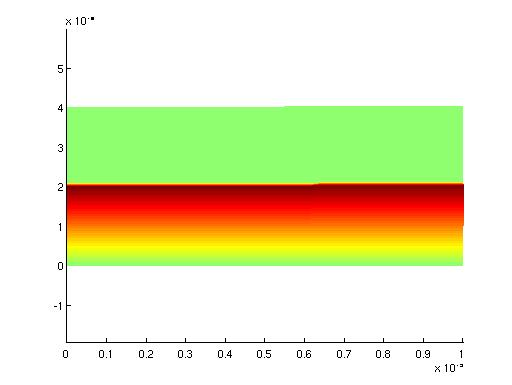
\includegraphics[height = 2in]{fig/mems_cant_em_dyn.jpg}
\caption{Dynamic mode of a MEMS cantilever beam}
\label{fig:MEMSCantileverBeamEMDynamic}
\end{figure}


\begin{verbatim}
Freq [Hz]   :2.791479e+07
            :3.452636e-11
Q           :4.042533e+17
\end{verbatim}

\clearpage
\subsubsection*{Solve for transfer function  (MATLAB)}
Once the mesh is defined, the next step is to solve the problem.
Since this script is identical to the mechanical case we will only
explain the parameters that are set.
\begin{itemize}

  \item{\textbf{Setting parameters:}}

\end{itemize}
The estimate for the center frequency should be obtained from the
previous dynamic eigenfrequency analysis. If model reduction is
required, only the value of \ttt{kmax} has to be set to a nonzero value.

\begin{figure}
\centering
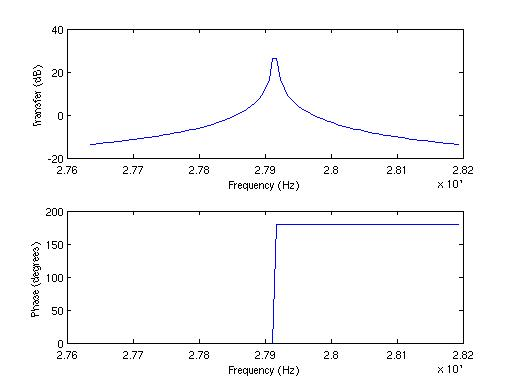
\includegraphics[height = 2in]{fig/mems_cant_em_tra.jpg}
\caption{Transfer function of a MEMS cantilever beam}
\label{fig:MEMSCantileverBeamEMTransfer}
\end{figure}



